% ============================================================
%  Meridian Capital - Asset Management Challenge 2026
%  Round 1 presentation (Beamer, 16:9). Compile with XeLaTeX, twice.
%  Files next to this one: Meridian-Capital-Official-Logo.png,
%  figures/pie_overall.pdf, pie_asset_type.pdf, pie_sector.pdf,
%  pie_region.pdf, cumulative-returns.pdf
% ============================================================
\documentclass[aspectratio=169,11pt,t]{beamer}
\usepackage{colortbl}

\usepackage{fontspec}
\usepackage{lmodern}
\usefonttheme{professionalfonts}
\setmainfont{DMSans}[Path=fonts/,Extension=.ttf,UprightFont=*-Regular,BoldFont=*-Bold,ItalicFont=*-Italic,BoldItalicFont=*-BoldItalic]
\setsansfont{DMSans}[Path=fonts/,Extension=.ttf,UprightFont=*-Regular,BoldFont=*-Bold,ItalicFont=*-Italic,BoldItalicFont=*-BoldItalic]
\renewcommand{\familydefault}{\sfdefault}
\usepackage{microtype}
\usepackage{booktabs,array,tabularx}
\usepackage{graphicx}
\usepackage{tikz}

% ---------- palette ----------
\definecolor{navy}{HTML}{0A2233}
\definecolor{ink}{HTML}{173242}
\definecolor{gold}{HTML}{A59577}
\definecolor{paper}{HTML}{F7F5EF}
\definecolor{muted}{HTML}{59666B}
\definecolor{line}{HTML}{D9DCD7}

\newcommand{\hd}[1]{\textcolor{navy}{\textbf{#1}}}
\newcommand{\smnote}[1]{{\footnotesize\color{muted}#1}}

% ---------- beamer theme ----------
\usetheme{default}
\usecolortheme{default}
\setbeamertemplate{navigation symbols}{}
\setbeamercolor{normal text}{fg=ink,bg=white}
\setbeamercolor{structure}{fg=navy}
\setbeamercolor{frametitle}{fg=navy}
\setbeamercolor{itemize item}{fg=gold}
\setbeamercolor{itemize subitem}{fg=gold}
\setbeamercolor{enumerate item}{fg=gold}
\setbeamertemplate{itemize item}[square]
\setbeamertemplate{itemize subitem}[square]
\setbeamerfont{itemize/enumerate body}{size=\normalsize}
\setbeamerfont{itemize/enumerate subbody}{size=\small}

% body, title and footer share the same side margins
\setbeamersize{text margin left=1.2cm,text margin right=1.2cm}

% frame title: serif, gold rule below
\setbeamertemplate{frametitle}{%
  \vspace{0.55em}
  \begin{beamercolorbox}[wd=\paperwidth,ht=2.0ex,dp=0.3ex,leftskip=1.2cm,rightskip=1.2cm]{frametitle}
    {\rmfamily\LARGE\color{navy}\insertframetitle}
  \end{beamercolorbox}
  \vspace{-1.0em}
  {\hspace{1.2cm}\color{gold}\rule{\dimexpr\paperwidth-2.4cm\relax}{0.8pt}}
}

% footer: MERIDIAN CAPITAL · AMC 2026, page number right
\setbeamertemplate{footline}{%
  \leavevmode\hbox{\begin{beamercolorbox}[wd=\paperwidth,ht=3ex,dp=1ex,leftskip=1.2cm,rightskip=1.2cm]{normal text}
    {\color{line}\hrule height 0.3pt}\vspace{2pt}
    {\fontsize{5}{6}\selectfont\color{muted}\textls[100]{MERIDIAN CAPITAL}\ ·\ AMC 2026}%
    \hfill{\fontsize{5}{6}\selectfont\color{navy}\insertframenumber\,/\,\inserttotalframenumber}
  \end{beamercolorbox}}%
}

% highlighted box
\usepackage[most]{tcolorbox}
\newtcolorbox{calloutbox}[1]{enhanced, colback=paper, colframe=paper,
  borderline west={2.5pt}{0pt}{gold}, boxrule=0pt, arc=0pt,
  left=10pt, right=8pt, top=6pt, bottom=6pt,
  title={#1}, fonttitle=\bfseries\small\raggedright, coltitle=navy, colbacktitle=paper,
  attach title to upper=\par\vspace{2pt}, before upper={\color{ink}\raggedright}}
\newenvironment{callout}[1]{\begin{calloutbox}{#1}}{\end{calloutbox}}

% big number tile: value, label, width
\newcommand{\kpi}[3]{%
  \begin{minipage}[t]{#3}\centering
  {\rmfamily\fontsize{22}{26}\selectfont\color{navy}#1}\\[3pt]
  {\scriptsize\color{gold}\textls[60]{\MakeUppercase{#2}}}
  \end{minipage}}

% compact list inside columns
\newcommand{\tight}{\setlength{\itemsep}{0.45em}\setlength{\parskip}{0pt}}

% ============================================================
\begin{document}

% ---------------------------- TITLE ----------------------------
{
\setbeamertemplate{footline}{}
\setbeamercolor{background canvas}{bg=paper}
\begin{frame}[plain]
\centering
\vspace*{0.1cm}

\includegraphics[width=5.2cm]{Meridian-Capital-Official-Logo.png}\par
\vspace{0.25cm}
{\color{gold}\rule{3cm}{0.8pt}}\par
\vspace{0.35cm}
{\rmfamily\fontsize{22}{26}\selectfont\color{navy}Strategic Asset Allocation\par}
\vspace{0.15cm}
{\scriptsize\color{gold}\textls[100]{ROUND 1 \,·\, ASSET MANAGEMENT CHALLENGE 2026}\par}
\vfill
{\footnotesize\color{navy}Alessia Battistella \ · \ Tze Qing Ginnie Lee \ · \ Katherine Lerner-Teves\\[1pt] Kyla Kaplan \ · \ Lorenzo Comi\par}
\vspace{0.15cm}
{\scriptsize\color{muted}USI \,·\, October 2026\par}
\vspace{0.2cm}
\end{frame}
}

% ---------------------------- AGENDA ----------------------------
\begin{frame}{Agenda}
\vspace{1.2em}
\begin{columns}[T]
\begin{column}{0.52\textwidth}
\begin{enumerate}\setlength{\itemsep}{0.8em}
\item Investment policy
\item Portfolio and allocation
\item Comparison with robust approaches
\item The backtest
\item Backtest protocol and robustness
\item Implementation
\end{enumerate}
\end{column}
\begin{column}{0.42\textwidth}
\begin{callout}{In one sentence}
A long-only portfolio of six ETFs for USD 100 million: 8\% target volatility, a 20\% maximum drawdown tolerance, and a mix chosen with inflation, high rates and energy-supply risk in mind.
\end{callout}
\end{column}
\end{columns}
\end{frame}

% ---------------------------- 1. POLICY ----------------------------
\begin{frame}{Market Outlook, October 2026}
\vspace{0.8em}
\begin{itemize}\setlength{\itemsep}{0.5em}
\item \textbf{Inflation is persistent} and interest rates are elevated
\item \textbf{The Fed has tightened again}, with further policy meetings ahead
\item \textbf{Long-term yields are high}, which can pressure equity valuations and bond prices
\item \textbf{Energy prices are high}, adding to inflation and supply risk
\item \textbf{Main risks:} persistent inflation, weaker growth and Middle East disruption
\item \textbf{EEMV adds non-US equity exposure} with a minimum-volatility approach; country and currency risks remain
\end{itemize}
\vfill
{\raggedright\tiny\color{muted}Sources: Federal Reserve, BLS, EIA, FRED. Detailed figures are in the report.\par}
\end{frame}
%------
\begin{frame}{Objective and Risk Budget}
\vspace{0.6em}
{\small Maximize estimated return at 8\% annual volatility, subject to our diversification limits.}
\vspace{1.3em}

\begin{columns}[T]
\begin{column}{0.31\textwidth}
\kpi{8.00\%}{Volatility, budget 7--9\%}{\linewidth}\\[0.8em]
{\footnotesize Last 60 monthly USD returns (Oct 2021--Sep 2026). Covariance $\times 12$; volatility $\times\sqrt{12}$.}
\end{column}
\begin{column}{0.31\textwidth}
\kpi{3.80\%}{1-month 95\% VaR, USD 3.8m}{\linewidth}\\[0.8em]
{\footnotesize $1.645\,\sigma/\sqrt{12}$ with $\sigma=8\%$. Assumes normal returns. Losses can exceed this estimate.}
\end{column}
\begin{column}{0.31\textwidth}
\kpi{-16.19\%}{Backtest max drawdown}{\linewidth}\\[0.8em]
{\footnotesize Largest fall from a month-end peak. Our tolerance is 20\%; losses can exceed it. We have no automatic stop-loss.}
\end{column}
\end{columns}
\end{frame}
%-----
\begin{frame}{Self-imposed Constraints}
\vspace{0.7em}
{\small The mandate requires long only and no leverage. We add five limits:}
\vspace{0.7em}

\small
\renewcommand{\arraystretch}{1.25}
\begin{tabularx}{\textwidth}{@{}>{\raggedright\arraybackslash}p{6.8cm} X@{}}
\toprule
\hd{Constraint} & \hd{Reason}\\
\midrule
At least \textbf{5\%} in each of five blocks: US equity (SPY+SCHD), EM equity (VWO+EEMV), DBC, VGSH, STIP & Keeps every block represented; individual ETFs can receive zero weight\\
At least \textbf{20\%} in VGSH + STIP & Retains a combined bond allocation\\
At most \textbf{35\%} of capital in one ETF & Limits dependence on a single fund\\
At most \textbf{40\%} of total risk from one ETF & Capital and risk weights differ, so we cap both\\
At most \textbf{65\%} of total risk from equities & Avoids relying only on the stock market\\
\bottomrule
\end{tabularx}
\end{frame}

% ---------------------------- 2. PORTFOLIO ----------------------------
\begin{frame}{The Portfolio: USD 100 million in six ETFs}
\vspace{0.7em}
\scriptsize
\renewcommand{\arraystretch}{1.15}
\begin{tabularx}{\textwidth}{@{}l >{\raggedright\arraybackslash}X r r >{\raggedright\arraybackslash}p{3.1cm}@{}}
\toprule
\hd{Ticker} & \hd{Fund} & \hd{Weight} & \hd{Risk share} & \hd{Role}\\
\midrule
STIP & iShares 0--5 Year TIPS Bond & 29.03\% & 6.23\% & Inflation-linked Treasuries\\
DBC  & Invesco DB Commodity Index & 26.95\% & 39.99\% & Broad commodity futures\\
SPY  & SPDR S\&P 500 ETF & 26.08\% & 40.00\% & US large-cap equity\\
EEMV & iShares MSCI EM Min Vol & 9.66\% & 8.62\% & EM equity, lower volatility\\
VGSH & Vanguard Short-Term Treasury & 5.00\% & 0.37\% & Short nominal Treasuries\\
SCHD & Schwab US Dividend Equity & 3.28\% & 4.79\% & US dividend equity\\
\midrule
\hd{Total} & & \hd{100.00\%} & \hd{100.00\%} & \\
\bottomrule
\end{tabularx}
\vspace{0.5em}

\smnote{Constrained mean--variance optimisation, long only. VWO is eligible but receives zero weight. Risk share = $w_i(\Sigma w)_i/(w^\top\Sigma w)$.}
\end{frame}

\begin{frame}{Capital Weights and Risk Shares}
\vspace{0.5em}
\begin{columns}[T]
\begin{column}{0.60\textwidth}
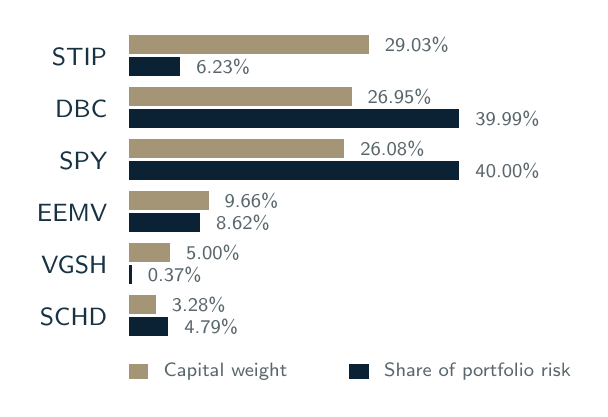
\begin{tikzpicture}[x=1cm,y=1cm]
\foreach \n/\c/\r [count=\i] in {STIP/29.03/6.23, DBC/26.95/39.99, SPY/26.08/40.00, EEMV/9.66/8.62, VGSH/5.00/0.37, SCHD/3.28/4.79}{
  \pgfmathsetmacro{\y}{-\i*0.66}
  \node[anchor=east,font=\small\color{ink}] at (0.55,\y) {\n};
  \fill[gold] (0.7,\y+0.04) rectangle ({0.7+\c*0.105},{\y+0.28});
  \node[anchor=west,font=\scriptsize\color{muted}] at ({0.78+\c*0.105},{\y+0.16}) {\c\%};
  \fill[navy] (0.7,\y-0.24) rectangle ({0.7+\r*0.105},{\y});
  \node[anchor=west,font=\scriptsize\color{muted}] at ({0.78+\r*0.105},{\y-0.12}) {\r\%};
}
\fill[gold] (0.7,-4.75) rectangle (0.95,-4.55);
\node[anchor=west,font=\scriptsize\color{muted}] at (1.02,-4.65) {Capital weight};
\fill[navy] (3.5,-4.75) rectangle (3.75,-4.55);
\node[anchor=west,font=\scriptsize\color{muted}] at (3.82,-4.65) {Share of portfolio risk};
\end{tikzpicture}
\end{column}
\begin{column}{0.36\textwidth}
\vspace{0.4em}
\begin{callout}{Reading the chart}
STIP is 29.03\% of capital but only 6.23\% of risk.\\[4pt]
SPY and DBC are 53.03\% of capital and 79.99\% of risk.\\[4pt]
\footnotesize\color{muted}We allow each ETF to contribute up to 40\% of portfolio risk.
\end{callout}
\end{column}
\end{columns}
\end{frame}

\begin{frame}{How the Weights Were Chosen}
\vspace{0.6em}
\begin{enumerate}\setlength{\itemsep}{0.65em}\small
\item \textbf{Inputs.} We estimate mean returns, volatilities and covariances from 60 monthly USD returns
\item \textbf{Objective.} The solver chooses all weights together to maximize estimated return at 8\% volatility, with long-only weights summing to 100\%
\item \textbf{Limits.} We require exposure to five blocks, a minimum bond allocation and caps on capital and risk shares
\item \textbf{Result.} SPY and DBC reach their 40\% risk caps; VGSH reaches its 5\% capital floor. The solver chooses the other weights within the remaining limits
\end{enumerate}
\vfill
{\footnotesize\color{muted}At the same 8\% volatility and risk-free rate, maximizing estimated return also maximizes estimated Sharpe. Future returns and correlations may differ from these estimates.\par}
\end{frame}

\begin{frame}{Allocation by Asset Type}
\vfill
\centering
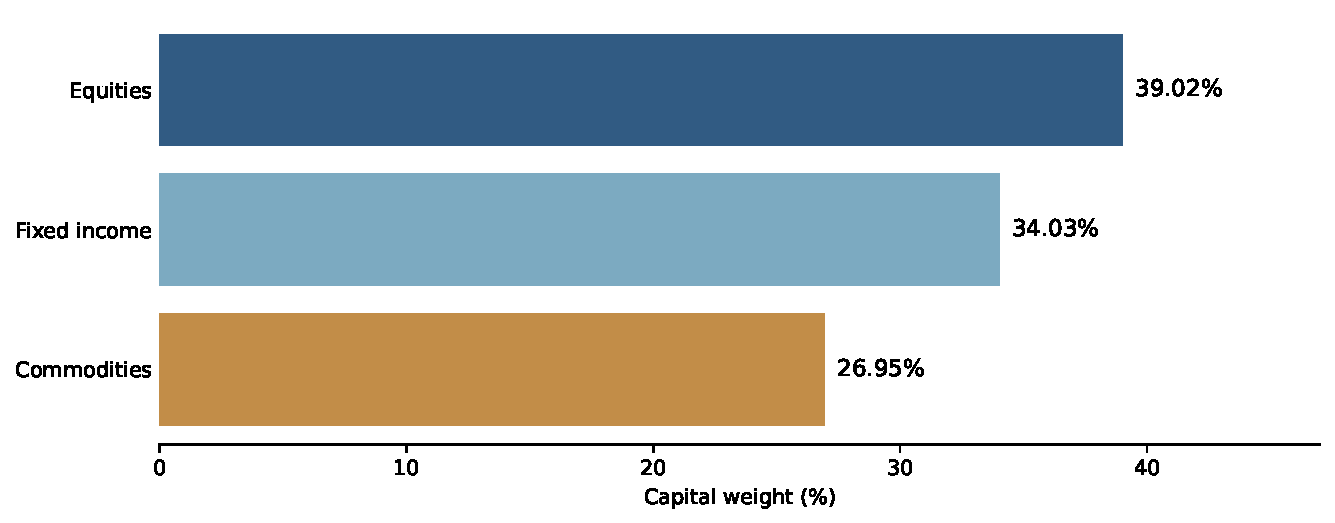
\includegraphics[width=0.85\textwidth,height=0.62\textheight,keepaspectratio]{asset-classes.pdf}\par
\vspace{0.6em}
{\small\itshape Capital is split across equities, commodities and short-term bonds.}\par
\vfill
\end{frame}

% ---------------------------- 3. ROBUST ----------------------------
\begin{frame}{Comparison with Robust Approaches}
\vspace{0.2em}
\begin{columns}[T]
\begin{column}{0.64\textwidth}
\footnotesize
\setlength{\tabcolsep}{2.4pt}
\renewcommand{\arraystretch}{1.18}
\arrayrulecolor{line}
\begin{tabular}{@{}l|rr|rr|rr@{}}
\toprule
& \multicolumn{2}{c|}{\hd{Our MVO}} & \multicolumn{2}{c|}{\hd{Equal weight}} & \multicolumn{2}{c}{\hd{Risk parity}}\\
\cmidrule(lr){2-3}\cmidrule(lr){4-5}\cmidrule(l){6-7}
ETF & Capital & Risk & Capital & Risk & Capital & Risk\\
\midrule
SPY  & 26.08\% & 40.00\% & 16.67\% & 27.74\% & 5.18\%  & 16.67\%\\
EEMV & 9.66\%  & 8.62\%  & 16.67\% & 18.21\% & 7.14\%  & 16.67\%\\
DBC  & 26.95\% & 39.99\% & 16.67\% & 19.98\% & 7.85\%  & 16.67\%\\
VGSH & 5.00\%  & 0.37\%  & 16.67\% & 1.79\%  & 47.65\% & 16.67\%\\
SCHD & 3.28\%  & 4.79\%  & 16.67\% & 28.32\% & 5.08\%  & 16.67\%\\
STIP & 29.03\% & 6.23\%  & 16.67\% & 3.95\%  & 27.09\% & 16.67\%\\
\midrule
Volatility & \multicolumn{2}{c|}{8.00\%} & \multicolumn{2}{c|}{7.80\%} & \multicolumn{2}{c}{3.75\%}\\
\bottomrule
\end{tabular}
\vspace{0.4em}

{\tiny\color{muted}Same six ETFs, Oct 2021--Sep 2026 covariance. Equal weight and risk parity use no additional MVO limits.}
\end{column}
\begin{column}{0.31\textwidth}
\begin{callout}{Where the rules disagree}
\footnotesize
\textbf{Equal weight:} SPY and SCHD generate about 56\% of the risk.\\[3pt]
\textbf{Risk parity:} 47.65\% in VGSH; volatility 3.75\%, below the band. Scaling to 8\% needs prohibited leverage.\\[3pt]
\textbf{Ours:} more risk to SPY and DBC (higher means, correlation 0.119), within the 40\% caps.
\end{callout}
\end{column}
\end{columns}
\end{frame}

% ---------------------------- 4. BACKTEST ----------------------------
\begin{frame}{The Backtest: How it was run}
\vfill
\begin{columns}[c]
\begin{column}{0.60\textwidth}
\centering
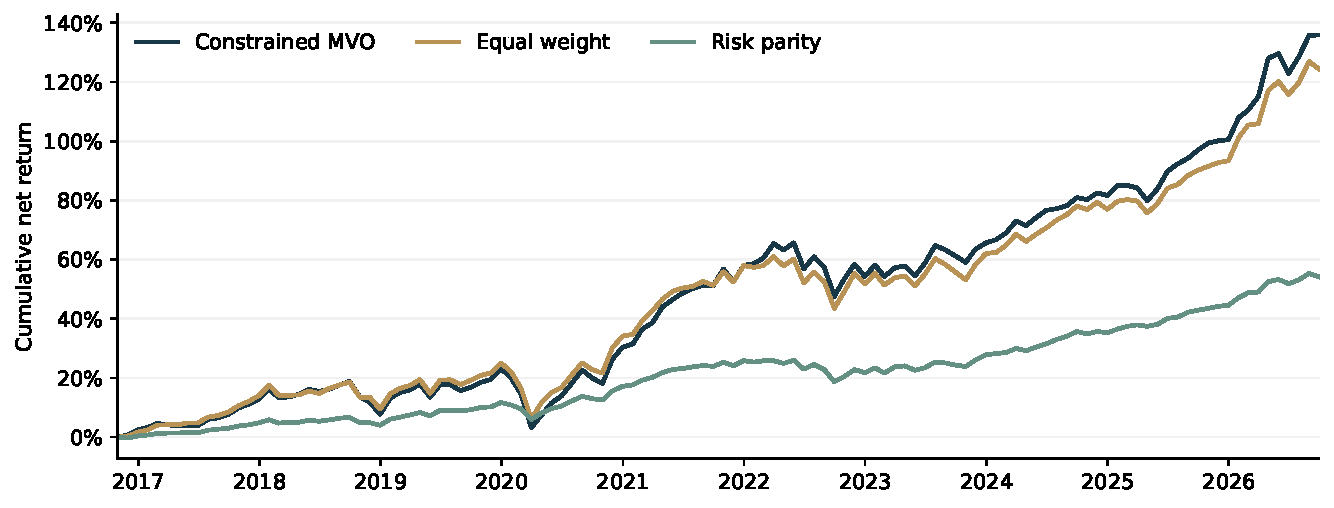
\includegraphics[width=\linewidth,height=0.78\textheight,keepaspectratio]{cumulative-returns.pdf}\par
{\tiny\color{muted}Cumulative net returns of the fixed target allocations. Retrospective illustration.}
\end{column}
\begin{column}{0.34\textwidth}
\begin{itemize}\tight\footnotesize
\item Nov 2016--Sep 2026, 119 monthly returns
\item Same target weights restored at each month-end
\item Net of 10 bp per dollar traded, including the initial investment
\item Weights fitted on Oct 2021--Sep 2026. Applying them to earlier history introduces look-ahead bias
\end{itemize}
\end{column}
\end{columns}
\vfill
\end{frame}

\begin{frame}{The Backtest: Performance and Risk}
\vspace{0.5em}
\centering
\kpi{9.04\%}{Annual return (MVO)}{0.26\textwidth}
\kpi{0.768}{Sharpe ratio}{0.26\textwidth}
\kpi{USD 235.9m}{Final value of USD 100m}{0.36\textwidth}
\par\vspace{0.7em}

\footnotesize
\renewcommand{\arraystretch}{1.2}
\begin{tabularx}{\textwidth}{@{}>{\raggedright\arraybackslash}X r r r r@{}}
\toprule
\hd{Fixed allocation} & \hd{CAGR} & \hd{Volatility} & \hd{Sharpe} & \hd{Max. drawdown}\\
\midrule
Constrained MVO & 9.04\% & 8.60\% & 0.768 & -16.19\%\\
Equal weight    & 8.49\% & 8.30\% & 0.731 & -15.17\%\\
Risk parity     & 4.46\% & 3.53\% & 0.561 & -5.81\%\\
\bottomrule
\end{tabularx}
\vspace{0.5em}

\raggedright\scriptsize
MVO's Sharpe is slightly higher than equal weight's. Risk parity had a smaller drawdown and volatility below the required band.
\end{frame}

% ---------------------------- 5. PROTOCOL ----------------------------
\begin{frame}{Backtest Protocol}
\vspace{0.5em}
\begin{columns}[T]
\begin{column}{0.56\textwidth}
\begin{itemize}\tight\footnotesize
\item \textbf{Design:} fixed target weights restored monthly, Nov 2016--Sep 2026.
\item \textbf{Data used to choose:} Oct 2021--Sep 2026 returns (60 months).
\item \textbf{Data held out:} none. History was also reviewed when choosing ETFs, limits and methods; fits before Nov 2016 or Nov 2021 are conditional checks only.
\item \textbf{Variations tried:} 17 method labels, 18 diversification subsets, 255-subset screens; then 108 constraint settings, 32 return-input scenarios, 33 volatility ceilings. The counts overlap. Earlier trials informed selection; we kept the final allocation after the later checks.
\end{itemize}
\end{column}
\begin{column}{0.39\textwidth}
\small
\renewcommand{\arraystretch}{1.2}
\begin{tabularx}{\linewidth}{@{}>{\raggedright\arraybackslash}X r@{}}
\toprule
Realised volatility & 8.60\%\\
Max drawdown & -16.19\%\\
Historical VaR (5\%) & 3.68\%\\
Backtested Sharpe & 0.768\\
Discounted Sharpe & \hd{0.384}\\
\bottomrule
\end{tabularx}
\vspace{0.4em}

\tiny{We chose a 50\% haircut to allow for selection bias, overlap between fitting and evaluation data, and uncertainty in expected returns.}
\end{column}
\end{columns}
\end{frame}

\begin{frame}{Robustness and Stress Tests}
\vspace{0.5em}
\begin{columns}[T]
\begin{column}{0.31\textwidth}
\begin{callout}{Sensitivity}
\footnotesize
Risk caps of 37.5\% / 42.5\% reallocate 3.64\% / 3.83\% of capital; 35\% / 45\% reallocate 7.10\% / 11.76\%.\\[3pt]
VGSH annual mean +1 pp: 28.84\% of capital reallocated. Under the original inputs, annual expected return is 6.38 bp lower. The bond split is sensitive to this input.
\end{callout}
\end{column}
\begin{column}{0.33\textwidth}
\raggedright
\footnotesize
\renewcommand{\arraystretch}{1.2}
\begin{tabularx}{\linewidth}{@{}>{\raggedright\arraybackslash}X r@{}}
\toprule
\hd{Scenario} & \hd{Return}\\
\midrule
2018 Q4 & -9.35\%\\
Feb--Mar 2020 & -13.82\%\\
2022 & -2.35\%\\
Growth shock & -11.89\%\\
Commodity reversal & -12.05\%\\
Inflation / rates shock & -2.49\%\\
\bottomrule
\end{tabularx}
\vspace{0.3em}

{\tiny\color{muted}Gross, selected weights. Periods differ in length; shocks have no assigned probability.}
\end{column}
\begin{column}{0.31\textwidth}
\begin{callout}{Tail and concentration}
\footnotesize
Expected shortfall (5\%): 5.67\%, USD 5.67m, against 3.68\% VaR.\\[3pt]
Rolling 12-month volatility ranged from 3.04\% to 16.51\%.\\[3pt]
SPY and DBC produced USD 57.61m and 49.13m of the USD 135.90m net profit.
\end{callout}
\end{column}
\end{columns}
\end{frame}

% ---------------------------- 6. IMPLEMENTATION ----------------------------
\begin{frame}{Implementation}
\vspace{0.3em}
{\small Bloomberg entry: 17 Oct 2026; prices: 16 Oct close (USD). Capital: USD 100m.}
\vspace{0.3em}

\footnotesize
\renewcommand{\arraystretch}{1.12}
\begin{tabularx}{\textwidth}{@{}l >{\raggedright\arraybackslash}X r r r@{}}
\toprule
\hd{Ticker} & \hd{ETF} & \hd{\# shares} & \hd{Price} & \hd{Weight}\\
\midrule
SPY  & State Street SPDR S\&P 500 ETF Trust & 34,169  & 763.25 & 26.08\%\\
EEMV & iShares MSCI Emerging Markets Min Vol Factor ETF & 133,610 & 72.30 & 9.66\%\\
DBC  & Invesco DB Commodity Index Tracking Fund & 798,756 & 33.74 & 26.95\%\\
VGSH & Vanguard Short-Term Treasury Index Fund ETF & 86,671 & 57.69 & 5.00\%\\
SCHD & Schwab U.S. Dividend Equity ETF & 95,488 & 34.35 & 3.28\%\\
STIP & iShares 0--5 Year TIPS Bond ETF & 288,630 & 100.58 & 29.03\%\\
\midrule
\hd{Total} & & & & \hd{100.00\%}\\
\bottomrule
\end{tabularx}
\vspace{0.4em}

\smnote{Opening market value USD 99,999,987.88; remaining cash USD 12.12. Shares are whole numbers, so actual weights differ slightly from the targets.}
\end{frame}

% ---------------------------- CLOSING ----------------------------
{
\setbeamertemplate{footline}{}
\setbeamercolor{background canvas}{bg=paper}
\begin{frame}[plain]
\centering
\vfill

\includegraphics[width=5cm]{Meridian-Capital-Official-Logo.png}\par
\vspace{0.4cm}
{\color{gold}\rule{3cm}{0.8pt}}\par
\vspace{0.4cm}
{\rmfamily\fontsize{22}{26}\selectfont\color{navy}Thank you\par}

\vfill
\end{frame}
}

\end{document}